\chapter{Tensor Algebra, Metrics, and the First Step to Space-Time}

This lecture marks a real threshold in the course. Leonard Susskind begins by warning us that the ``theoretical minimum'' has ceased to be verbal; from this point on the minimum already demands patience with calculation. We therefore proceed the way the lecture proceeds: first by reviewing how tensor components transform, then by building tensor algebra from those rules, then by introducing the metric as the object that measures distance, and only after that by turning to flat space, special relativity, and a first time-dependent cosmological metric. These companion notes follow Susskind's lecture closely and preserve selected documentary board frames associated with the lecture curation by LazyingArt LLC and Video2Book.

\section{Covariant and Contravariant Review}

The lecture begins with a deliberate reset. We are not going to define vectors geometrically at first. We are going to define them by how their components transform when we pass from one coordinate system to another.

Let \(x^m\) and \(y^m\) be two coordinate systems. Susskind's convention is that coordinates themselves carry upper indices. With that convention in place, the transformation rules are easy to remember: lower indices transform with \(\partial x/\partial y\), and upper indices transform with \(\partial y/\partial x\).

For a covariant object,
\begin{equation}
V_m(y)=\frac{\partial x^n}{\partial y^m}V_n(x).
\end{equation}
For a contravariant object,
\begin{equation}
W^m(y)=\frac{\partial y^m}{\partial x^n}W^n(x).
\end{equation}

The point is not decorative. A list of numbers is not a vector merely because we can draw an arrow from it. Susskind's example is intentionally blunt: temperature, pressure, and humidity give three numbers, but those numbers do not transform as components of a vector. They are just three scalars. What makes an object a vector is its transformation law.

The two archetypes in the lecture come directly from the chain rule:
\begin{align}
\frac{\partial \phi}{\partial y^m}
&=
\frac{\partial \phi}{\partial x^n}
\frac{\partial x^n}{\partial y^m}, \\
dy^m
&=
\frac{\partial y^m}{\partial x^n}\,dx^n.
\end{align}
Thus gradients transform covariantly, and differential displacements transform contravariantly.

\subsection{Question \& Answer}

\paragraph{Question.} If an object satisfies one of these vector transformation laws, must it satisfy the other one too?

\paragraph{Answer.} Not at this stage. The lecture insists on keeping the two kinds of objects separate at first. A gradient,
\[
\frac{\partial \phi}{\partial x^m},
\]
is a covariant vector. A differential displacement,
\[
dx^m,
\]
is a contravariant vector. They are different kinds of components. Only later, once the metric has been introduced, do we gain a natural way to pass from one version to the other and think of them as two representations of the same underlying vector.

\section{From Vectors to General Tensors}

Once the one-index pattern is clear, the generalization is mechanical. Every index transforms, and each index brings along its own Jacobian factor.

For a rank-two covariant tensor,
\begin{equation}
T_{mr}(y)=
\frac{\partial x^n}{\partial y^m}
\frac{\partial x^s}{\partial y^r}
T_{ns}(x).
\end{equation}
For a mixed tensor with one upper and one lower index,
\begin{equation}
T^m{}_{n}(y)=
\frac{\partial y^m}{\partial x^s}
\frac{\partial x^r}{\partial y^n}
T^s{}_{r}(x).
\end{equation}

This is the pattern Susskind wants us to internalize: indices are what transform. A tensor is not defined first by a picture in space and only later by equations. It is defined by the equations.

The next decisive move is contraction. If we identify one upper index and one lower index and sum over them, the rank drops. For example,
\begin{equation}
T^m{}_{m}=T^1{}_{1}+T^2{}_{2}+T^3{}_{3}+\cdots
\end{equation}
has no free indices left. The lecture emphasizes that such an object should be expected to be a scalar, and indeed it is.

\paragraph{Why contraction works.} In the mixed transformation law, setting the upper and lower indices equal produces a factor
\begin{equation}
\frac{\partial x^r}{\partial y^m}\frac{\partial y^m}{\partial x^s}
=
\delta^r{}_{s},
\end{equation}
the Kronecker delta. The transformation factors collapse, and one is left with the same contracted quantity in the new coordinates. This is why \(T^m{}_{m}\) is a scalar.

More generally, contraction of one upper and one lower index lowers the rank by two and produces another tensor. As a familiar example, if \(v^m\) is contravariant and \(w_m\) is covariant, then
\begin{equation}
v^m w_m
\end{equation}
is a scalar: the inner product.

This is the first real payoff of tensor algebra. Contraction is not merely notation. It manufactures coordinate-independent quantities out of objects whose individual components do depend on coordinates.

\section{The Metric Tensor as Distance}

The first rank-two tensor in the lecture with immediate geometric content is the metric tensor. If two neighboring points are separated by the differential displacement \(dx^m\), then the squared distance between them is
\begin{equation}
ds^2=g_{mn}(x)\,dx^m dx^n.
\end{equation}

This is already a contraction: two contravariant indices from \(dx^m dx^n\), and two covariant indices from \(g_{mn}\). No free index remains, so \(ds^2\) is a scalar.

But now comes the real test. Is \(g_{mn}\) genuinely a tensor? The lecture answers this exactly the right way: rewrite the same line element in another coordinate system.

We write
\begin{equation}
dx^m=\frac{\partial x^m}{\partial y^r}\,dy^r,
\end{equation}
and substitute twice:
\begin{align}
ds^2
&=g_{mn}(x)\,dx^m dx^n \\
&=
g_{mn}(x)
\frac{\partial x^m}{\partial y^r}
\frac{\partial x^n}{\partial y^s}
dy^r dy^s.
\end{align}
Now define the coefficient of \(dy^r dy^s\) to be the metric components in the \(y\)-system:
\begin{equation}
g_{rs}(y)=
\frac{\partial x^m}{\partial y^r}
\frac{\partial x^n}{\partial y^s}
g_{mn}(x).
\end{equation}
This is exactly the covariant rank-two transformation law. So the metric tensor really is a tensor.

\paragraph{Worked derivation.} The logic is worth stating in the clipped form in which the lecture presents it:
\begin{enumerate}
\item Start from \(ds^2=g_{mn}(x)\,dx^m dx^n\).
\item Rewrite each \(dx\) in terms of \(dy\).
\item Collect the coefficient of \(dy^r dy^s\).
\item Call that coefficient \(g_{rs}(y)\).
\item Read off the tensor transformation law.
\end{enumerate}

\subsection{Question \& Answer}

\paragraph{Question.} Is \(ds^2\) ``the same regardless of the coordinates''?

\paragraph{Answer.} Yes, but only in the precise sense used in the lecture: we are not comparing two independent formulas that happen to agree. We are rewriting one and the same scalar interval in different coordinates. That is exactly what forces the relation between \(g_{mn}(x)\) and \(g_{rs}(y)\). The invariance of \(ds^2\) is not an extra miracle after the fact; it is the starting point of the derivation.

\section{Metric as Matrix, Inverse Metric, and Raising/Lowering}

At a fixed point and in a fixed coordinate system, the collection of components \(g_{mn}\) may be regarded as a matrix. Strictly speaking the metric is a tensor, not a matrix; but the lecture repeatedly moves back and forth between these two languages, and we should preserve that interplay.

\begin{figure}[htbp]
\centering

\includegraphics[width=0.78\textwidth]{lecture_04_figure_04.png}
\caption{Metric tensor as matrix and inverse}
\end{figure}

In that matrix language,
\begin{equation}
g_{mn}\leftrightarrow
\begin{pmatrix}
g_{11} & g_{12} & g_{13} & \cdots \\
g_{21} & g_{22} & g_{23} & \cdots \\
g_{31} & g_{32} & g_{33} & \cdots \\
\vdots & \vdots & \vdots & \ddots
\end{pmatrix}.
\end{equation}
The lecture assumes two further facts about the metric:
\begin{itemize}
\item it is symmetric,
\item it has an inverse.
\end{itemize}

The matrix statement is
\begin{equation}
g^{-1}g=I,
\end{equation}
and in index notation this becomes
\begin{equation}
g^{mr}g_{rn}=\delta^m{}_{n}.
\end{equation}
The upper-index components \(g^{mn}\) are not a new independent tensor carrying new information. They are the components of the inverse matrix to \(g_{mn}\), written in tensor notation.

\begin{figure}[htbp]
\centering

\includegraphics[width=0.72\textwidth]{lecture_04_figure_02.png}
\caption{Inverse metric contraction identity}
\end{figure}

The lecture explicitly pauses here to state a theorem: if we invert the matrix of metric components, the resulting collection of components is itself a tensor, now with contravariant indices. We therefore write \(g^{mn}\) and call it the metric with contravariant components.

\subsection{Question \& Answer}

\paragraph{Question.} Can the metric tensor fail to have an inverse?

\paragraph{Answer.} A general tensor can fail to have an inverse, but in the lecture Susskind takes as a rule that the metric does not. He attributes this to the symmetry of the metric and to the absence of zero eigenvalues. The full proof is deferred, and the notes should not pretend otherwise. At this stage we use the invertibility of the metric as part of the working setup of the geometry.

\begin{figure}[htbp]
\centering

\includegraphics[width=0.72\textwidth]{lecture_04_figure_03.png}
\caption{Inverse metric relation}
\end{figure}

A simple example from the lecture is the plane in polar coordinates:
\begin{equation}
ds^2=dr^2+r^2 d\theta^2.
\end{equation}
If \(r\) is the first coordinate and \(\theta\) the second, then
\begin{equation}
g_{11}=1,\qquad g_{22}=r^2,
\end{equation}
and the inverse metric is
\begin{equation}
g^{11}=1,\qquad g^{22}=\frac{1}{r^2}.
\end{equation}
For a diagonal matrix the inverse is immediate: we simply invert each diagonal entry.

\subsection{Question \& Answer}

\paragraph{Question.} Why may we take the metric to be symmetric?

\paragraph{Answer.} Because only the symmetric part contributes to the quadratic form \(ds^2\). The cross terms are
\begin{equation}
g_{12}\,dx^1 dx^2+g_{21}\,dx^2 dx^1
=
(g_{12}+g_{21})\,dx^1 dx^2,
\end{equation}
since \(dx^1 dx^2=dx^2 dx^1\). The antisymmetric part drops out. Thus there is no loss of generality, for the purposes of the line element, in taking the metric symmetric. This is partly convention, but it is a convention that exactly matches the physics carried by \(ds^2\).

Now the metric begins to do real work. Given a contravariant vector \(V^m\), we define its covariant components by
\begin{equation}
V_n=g_{nm}V^m.
\end{equation}
Conversely,
\begin{equation}
V^m=g^{mn}V_n.
\end{equation}
Likewise, for a rank-two tensor,
\begin{equation}
T^m{}_{n}=g^{mr}T_{rn}.
\end{equation}
This is the operation of raising and lowering indices.

The lecture then applies the same idea to the differential displacement:
\begin{equation}
dx_m=g_{mn}\,dx^n.
\end{equation}

\begin{figure}[htbp]
\centering

\includegraphics[width=0.76\textwidth]{lecture_04_figure_05.png}
\caption{Lowering an index with the metric}
\end{figure}

Here the blackboard contains a misleading equals sign in the first line, and Susskind later corrects it. The right way to present the step is as a contraction, not as a literal equality between two differently indexed expressions. With that correction made, the calculation is clean:
\begin{align}
dx^m dx_m
&=
dx^m\bigl(g_{mn}dx^n\bigr) \\
&=
g_{mn}\,dx^m dx^n \\
&=
ds^2.
\end{align}
So the same squared distance can be written in three equivalent ways:
\begin{equation}
ds^2=g_{mn}\,dx^m dx^n=dx^m dx_m=g^{mn}dx_m dx_n.
\end{equation}

This is the first serious payoff of the inverse metric. Once the metric is known, upper and lower components may be treated as two faithful representations of the same geometric object.

\section{Tensor Equalities and the End of Tensor Algebra}

The lecture closes the algebraic half of the subject with several sharp warnings and one powerful principle.

First, tensors may be added only if they are of the same type. It makes sense to add \(T_{mn}\) and \(W_{mn}\). It does not make sense to add an object with two lower indices to one with two upper indices and expect the result to transform cleanly. The index structure is part of the identity of the tensor.

Second, if a tensor is zero in one coordinate system, then it is zero in every coordinate system. This follows immediately from the transformation laws: the transformed components are built from Jacobian factors multiplying the original components. If the original components all vanish, the transformed ones vanish too.

Third, and more generally, if two tensors are equal in one coordinate system, they are equal in all coordinate systems. The proof is only one line longer: if
\[
T=W
\]
in one coordinate system, then
\[
T-W=0
\]
there. But a zero tensor is zero in every coordinate system, so \(T=W\) everywhere. This is one of the central powers of tensor language. A tensor equation is a geometric fact, not a coordinate accident.

At this point Susskind briefly turns toward tensor calculus and then deliberately stops. Ordinary derivatives of tensor components do not, in general, transform as tensor components. Something more subtle is needed, and that subject is postponed to the next lecture. The postponement matters. It clears the deck and lets the lecture pivot cleanly from space to space-time.

\section{Flat Space, Cartesian Frames, and the Pivot to Space-Time}

Before entering space-time, the lecture re-enters through ordinary flat space. Even if we restrict attention to Cartesian coordinates, there is still more than one Cartesian coordinate system. We may rotate the axes. We may translate them. These are coordinate transformations, although they are not curved or curvilinear ones.

In two-dimensional Cartesian coordinates the metric has the familiar form
\begin{equation}
ds^2=(dx^1)^2+(dx^2)^2=\delta_{mn}\,dx^m dx^n.
\end{equation}
Within this restricted Cartesian class, the distinction between upper and lower indices disappears: the metric is just the identity. The lecture does add a caution here. Writing \(\delta_{mn}\) with both indices downstairs is harmless in this restricted setting, but it is not the right fully tensorial notation once we move to general coordinate systems.

\begin{figure}[htbp]
\centering

\includegraphics[width=0.82\textwidth]{lecture_04_figure_06.png}
\caption{Flat line element and skew grid}
\end{figure}

The geometric lesson of this stage is that Cartesian-to-Cartesian transformations are precisely those that preserve the Euclidean form of the interval. They preserve the form of Pythagoras' theorem.

To make that board picture easier to read in finished notes, it is useful to redraw the geometry schematically.

\begin{figure}[htbp]
\centering
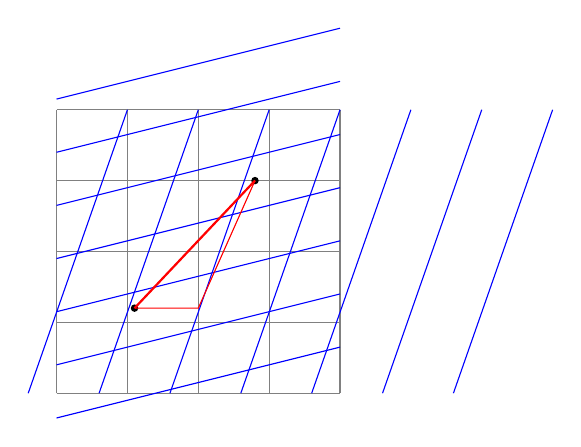
\begin{tikzpicture}[scale=0.9]
\draw[step=1,gray] (0,0) grid (4,4);

\foreach \k in {-1,0,1,2,3,4,5}
  \draw[blue] (\k+0.6,0) -- (\k+2.0,4);

\foreach \k in {-1,0,1,2,3,4,5}
  \draw[blue] (0,0.75*\k+0.4) -- (4,0.75*\k+1.4);

\fill (1.1,1.2) circle (1.5pt);
\fill (2.8,3.0) circle (1.5pt);
\draw[thick,red] (1.1,1.2) -- (2.8,3.0);
\draw[red] (1.1,1.2) -- (2.0,1.2) -- (2.8,3.0);
\end{tikzpicture}
\caption{Schematic redraw of the flat-plane picture: two coordinate descriptions of the same plane, with a highlighted interval whose Euclidean length is preserved.}
\end{figure}

Now comes the special-relativistic pivot. A naive Euclidean guess for one time and one space dimension would be
\[
dt^2+dx^2.
\]
But this is not the invariant quantity preserved by Lorentz transformations. The invariant interval is
\begin{equation}
d\tau^2=dt^2-dx^2.
\end{equation}
In three spatial dimensions,
\begin{equation}
d\tau^2=dt^2-dx^2-dy^2-dz^2.
\end{equation}

The lecture pauses over units because the point matters physically. Setting \(c=1\) is not a trick of laziness. It is the natural choice that puts time and space in the same units, just as one would not measure one spatial coordinate in feet and another in inches if the goal were to write rotationally natural formulas.

Special relativity is then described in the most economical way possible: it is the theory of coordinate transformations that preserve this indefinite interval.

\section{General Space-Time Metric and the First Cosmological Example}

From here the transition is immediate. Space-time has four coordinates, and the lecture now switches from Latin to Greek indices:
\[
x^\mu,\qquad \mu=0,1,2,3,
\]
with \(x^0\) denoting the time coordinate.

The generalization of the special-relativistic interval is exactly what the earlier tensor algebra suggests:
\begin{equation}
d\tau^2=g_{\mu\nu}(x)\,dx^\mu dx^\nu.
\end{equation}
At this level one does not yet need genuine curvature or gravitation. One can obtain nontrivial coefficients already by introducing nontrivial coordinates into flat space-time. What matters first is that the metric tensor has now become a space-time object.

The flat special case is Minkowski space. In Minkowski coordinates the metric is
\begin{equation}
\eta_{\mu\nu}=
\mathrm{diag}(1,-1,-1,-1),
\end{equation}
and therefore
\begin{equation}
d\tau^2=\eta_{\mu\nu}\,dx^\mu dx^\nu.
\end{equation}
In these coordinates the inverse is the same matrix,
\begin{equation}
\eta^{\mu\nu}=\eta_{\mu\nu},
\end{equation}
because the diagonal entries are \(\pm1\).

The lecture stresses that almost all of the tensor rules remain unchanged in space-time. Covariant and contravariant indices transform exactly as before. The new ingredient is the signature of the metric. In the convention used here there is one positive and three negative directions.

\subsection{Question \& Answer}

\paragraph{Question.} What does it mean, in the language of the metric, to say that space-time is expanding?

\paragraph{Answer.} It means that the metric coefficients depend on time in such a way that spatial separations at fixed coordinate differences change with time. The lecture writes this somewhat loosely as a diagonal metric with entries \(1,-A(t),-A(t),-A(t)\), but because the interval is described with a squared spatial factor, the clean first-pass normalization is
\begin{equation}
d\tau^2=dt^2-a^2(t)\bigl(dx^2+dy^2+dz^2\bigr).
\end{equation}
Here \(a(t)\) is the scale factor. If \(a(t)\) grows with time, then the space-time is expanding.

Susskind does not yet analyze curvature here. He builds intuition by analogy with two-dimensional metrics. On the plane in polar coordinates,
\begin{equation}
ds^2=dr^2+r^2 d\theta^2.
\end{equation}
If we replace \(r^2\) by \(\sin^2 r\), we obtain the metric of a sphere:
\begin{equation}
ds^2=dr^2+\sin^2 r\,d\theta^2.
\end{equation}
If instead we use an exponentially growing coefficient,
\begin{equation}
ds^2=dr^2+e^{2r}d\theta^2,
\end{equation}
we obtain a horn-like surface. The point of these examples is not to compute curvature yet, but to learn how the dependence of the metric coefficients on position changes the geometry.

The same reasoning is then carried back to space-time. In the cosmological metric, the role played by \(r\) in the surface analogy is now played by \(t\). As time changes, the geometry of space changes. That is what the lecture means, at this stage, by an expanding universe.

\section{Summary}

This lecture does two jobs at once. First, it completes the minimum tensor algebra needed for general relativity: transformation laws, mixed tensors, contraction, the metric, its inverse, and the raising and lowering of indices. Second, it uses exactly that machinery to pivot from ordinary space to space-time. Flat Euclidean space leads to Minkowski space, and Minkowski space leads naturally to the general line element
\[
d\tau^2=g_{\mu\nu}(x)\,dx^\mu dx^\nu.
\]
The next lecture will supply the missing step that has been deliberately deferred here: tensor calculus, curvature, and the first real encounter with Einstein's equations.